\documentclass[12 pt]{article}
\usepackage[utf8]{inputenc}
\usepackage{matlab-prettifier}
\usepackage[portuguese]{babel}
\usepackage{indentfirst}
\usepackage{graphicx}
\usepackage{float}
\usepackage{subcaption}
\usepackage[font=small,labelfont=bf]{caption}
\definecolor{mygreen}{RGB}{28,172,0} % color values Red, Green, Blue
\definecolor{myyellow}{rgb}{1.0, 1.0, 0.8}
\usepackage{mathtools}
\usepackage{multirow}
\usepackage{comment}
\usepackage{xcolor}
\usepackage{colortbl}
\usepackage[normalem]{ulem}               % to striketrhourhg text
\usepackage{amsmath}
\usepackage{amsfonts}
\usepackage{hyperref}
\usepackage{tcolorbox}
\newcommand\redout{\bgroup\markoverwith
{\textcolor{red}{\rule[0.5ex]{2pt}{0.8pt}}}\ULon}
\renewcommand{\lstlistingname}{Código}% Listing -> Algorithm
\renewcommand{\lstlistlistingname}{Lista de \lstlistingname s}% List of Listings -> List of Algorithms

\usepackage[top=3cm,left=2cm,bottom=2cm, right=2cm]{geometry}
\usepackage{tikz}
\usetikzlibrary{decorations.pathreplacing}


% Configuração para destacar a sintaxe do Python
\lstset{ 
    language=Python,                     % A linguagem do código
    backgroundcolor=\color{myyellow}, % A cor do fundo 
    basicstyle=\ttfamily\footnotesize,   % O estilo do texto básico
    keywordstyle=\color{blue},           % Cor das palavras-chave
    stringstyle=\color{red},             % Cor das strings
    commentstyle=\color{mygreen},          % Cor dos comentários
    numbers=left,                        % Números das linhas à esquerda
    numberstyle=\tiny\color{gray},       % Estilo dos números das linhas
    stepnumber=1,                        % Número de linhas entre os números das linhas
    frame=single,                        % Moldura ao redor do código
    breaklines=true,                     % Quebra automática das linhas longas
    captionpos=t,                        % Posição da legenda
    showstringspaces=false               % Não mostra espaços em branco nas strings
    extendedchars=true,
    literate={º}{{${ }^{\underline{o}}$}}1 {á}{{\'a}}1 {à}{{\`a}}1 {ã}{{\~a}}1 {é}{{\'e}}1 {É}{{\'E}}1 {ê}{{\^e}}1 {ë}{{\"e}}1 {í}{{\'i}}1 {ç}{{\c{c}}}1 {Ç}{{\c{C}}}1 {õ}{{\~o}}1 {ó}{{\'o}}1 {ô}{{\^o}}1 {ú}{{\'u}}1 {â}{{\^a}}1 {~}{{$\sim$}}1
}


\title{%
\textbf{\huge Universidade Federal do Rio de Janeiro} \par
\textbf{\LARGE Instituto Alberto Luiz Coimbra de Pós-Graduação e Pesquisa de Engenharia} \par


\includegraphics[width=8cm]{COPPE UFRJ.png} \par

\textbf{Programa de Engenharia de Sistemas e Computação} \par

CPS863 - Aprendizado de Máquina  \par

Prof. Dr. Edmundo de Souza e Silva (PESC/COPPE/UFRJ)\par

\vspace{1\baselineskip}
\textbf{\textit{Lista de Exercícios 1b}} \par
}

\author{Luiz Henrique Souza Caldas\\email: lhscaldas@cos.ufrj.br}

\date{\today}

\begin{document}
\maketitle


\section*{Questão 1}

Este exercício foi feito em classe no dia 10/Out/2024. A lista contém as questões resolvidas e ainda
alguns itens a mais. Faça a lista e complete as questões que faltaram.

Este exercício é motivado pelo trabalho em \url{https://ieeexplore.ieee.org/document/9006548},
Seção H (Leveraging spatio-temporal correlation across homes). O problema foi simplificado neste
exercício.

Imagine que dispomos de um classificador implementado em roteadores residenciais de um provedor
de Internet (ISP). A cada janela de tempo (por exemplo a cada 5 minutos) o classificador do roteador
$i$ fornece como saída uma dentre 2 possibilidades: (a) existe um ataque DDoS acontecendo a partir da
residência do roteador $i$, nesta janela de tempo; (b) não há ataque acontecendo a partir da residência
do roteador $i$ nesta janela.

A cada 5 minutos o ISP amostra o resultado de $M$ roteadores escolhidos de forma aleatória dentre
todos os roteadores da sua base que, para todos os efeitos deste problema, pode ser considerada como
muito grande (infinita). O objetivo do ISP é determinar, a partir das $M$ amostras coletadas, se
um ataque aconteceu ou não durante a janela de tempo amostrada. Em outras palavras, o ISP quer
determinar a possibilidade de uma das seguintes hipóteses serem verdadeiras: $h_a$ (há um ataque DDoS
acontecendo na rede do ISP na janela amostrada) ou $h_b$ que é a hipótese complementar.

O ISP conhece o classificador usado em cada roteador residencial, e sabe que o resultado não é
100\% confiável. Portanto, ele usará correlação espacial conforme sugerido no artigo acima e explicado
em classe.

No que se segue usaremos algumas definições comuns que podem ser encontradas em
\url{https://en.wikipedia.org/wiki/Confusion_matrix} (ver também a figura em \url{https://en.wikipedia.org/wiki/Confusion_matrix}).

\subsection*{Notação:}

\begin{itemize}
    \item $M$: número de roteadores amostrados (em uma janela de tempo);
    \item Inf: variável aleatória (va) indicando se a residência é um “bot”, isto é, está ou não infectada.
    $P[\text{Inf}]$ ($P[\overline{\text{Inf}}]$) é a probabilidade de uma residência estar infectada (não estar infectada);
    \item TPR: (true positive rate ou hit rate) taxa de acerto do classificador, ou probabilidade do classificador corretamente sinalizar um ataque, dado que um ataque está acontecendo no ISP (Nota: obviamente somente residências infectadas podem gerar um ataque quando ele ocorre);
    \item FPR: (false positive rate) ou probabilidade do classificador do roteador residencial erradamente sinalizar um ataque a partir da residência;
    \item $L$: variável aleatória indicadora $L = 1$ se o roteador alarma, $L = 0$, caso contrário;
    \item $P[h_a]$: probabilidade de ocorrer um ataque DDoS no ISP em uma janela de tempo. (Se você tem algum conhecimento prévio sobre ataques, talvez possa estimar o $P[h_a]$).
\end{itemize}

Suponha que, em uma determinada janela de tempo, das $M$ amostras coletadas, $V$ roteadores
sinalizaram que um ataque estava ocorrendo na janela (e então $M - V$ roteadores sinalizaram que
tudo estava normal nas suas respectivas residências). Suponha ainda que um ataque ocorre em um
intervalo independentemente das infecções nas residências.

Para os seus cálculos, suponha que: TPR = 0.8, FPR = 0.1, $P[\text{Inf}] = 0.2$. Como você
não tem conhecimento prévio sobre $P[h_a]$, suponha inicialmente que $P[h_a] = P[h_b] = 0.5$, $V = 20$, $M = 200$.

\vspace{1\baselineskip}
Responda as seguintes perguntas, mas só substitua os valores no final:

\begin{enumerate}
    \item Suponha que um ataque esteja ocorrendo. Calcule $P[L = 1|\text{Inf}, h_a]$ e $P[L = 1|\overline{\text{Inf}}, h_a]$, e então $P[L = 1|h_a]$ e $P[L = 0|h_a]$.
    
    \begin{tcolorbox}[colback=white, colframe=black, title=Resposta:]
Se o ataque está ocorrendo, temos:
$$
P[L = 1|\text{Inf}, h_a] = TPR = 0.8
$$
e
$$
P[L = 1|\overline{\text{Inf}}, h_a] = FPR = 0.1
$$

Podemos calcular \( P[L = 1|h_a] \) pela lei total da probabilidade:
$$
P[L = 1|h_a] = P[L = 1|\text{Inf}, h_a] \cdot P[\text{Inf}] + P[L = 1|\overline{\text{Inf}}, h_a] \cdot P[\overline{\text{Inf}}]
$$

Substituindo os valores:
$$
P[L = 1|h_a] = 0.8 \cdot 0.2 + 0.1 \cdot 0.8 = 0.16 + 0.08 = 0.24
$$

Agora, \( P[L = 0|h_a] \) é simplesmente o complementar de \( P[L = 1|h_a] \):
$$
P[L = 0|h_a] = 1 - P[L = 1|h_a] = 1 - 0.24 = 0.76
$$
    
    \end{tcolorbox}

    \item Suponha que um ataque não esteja ocorrendo. Calcule $P[L = 1|\text{Inf}, h_b]$ e $P[L = 1|\overline{\text{Inf}}, h_b]$, e então $P[L = 1|h_b]$ e $P[L = 0|h_b]$.
    
    \begin{tcolorbox}[colback=white, colframe=black, title=Resposta:]

    Se um ataque não está ocorrendo, temos:
    $$
    P[L = 1|\text{Inf}, h_b] = FPR = 0.1
    $$
    e
    $$
    P[L = 1|\overline{\text{Inf}}, h_b] = FPR = 0.1
    $$
    
    Podemos calcular \( P[L = 1|h_b] \) usando a lei total da probabilidade:
    $$
    P[L = 1|h_b] = P[L = 1|\text{Inf}, h_b] \cdot P[\text{Inf}] + P[L = 1|\overline{\text{Inf}}, h_b] \cdot P[\overline{\text{Inf}}]
    $$
    
    Substituindo os valores:
    $$
    P[L = 1|h_b] = 0.1 \cdot 0.2 + 0.1 \cdot 0.8 = 0.02 + 0.08 = 0.10
    $$
    
    Agora, \( P[L = 0|h_b] \) é o complementar de \( P[L = 1|h_b] \):
    $$
    P[L = 0|h_b] = 1 - P[L = 1|h_b] = 1 - 0.10 = 0.90
    $$
    
\end{tcolorbox}

    \item Calcule $P[D|h_a]$ em função de $V$ e $M$ (Likelihood).
    
    \begin{tcolorbox}[colback=white, colframe=black, title=Resposta:]

Sabemos que \( D \) representa os dados observados, isto é, \( V \) roteadores sinalizando um ataque de um total de \( M \) roteadores.

A probabilidade \( P[D|h_a] \) pode ser modelada como uma distribuição binomial, onde \( V \) roteadores sinalizam um ataque dado que um ataque realmente está ocorrendo (\( h_a \)):

$$
P[D|h_a] = \binom{M}{V} (P[L = 1|h_a])^V (P[L = 0|h_a])^{M-V}
$$

Substituindo \( P[L = 1|h_a] = 0.24 \) e \( P[L = 0|h_a] = 0.76 \):

$$
P[D|h_a] = \binom{M}{V} (0.24)^V (0.76)^{M-V}
$$

\end{tcolorbox}
\newpage

    \item Calcule $P[D|h_b]$ em função de $V$ e $M$ (Likelihood).
    
    \begin{tcolorbox}[colback=white, colframe=black, title=Resposta:]

De forma similar à Pergunta 3, modelamos \( P[D|h_b] \) como uma distribuição binomial. Agora, \( h_b \) indica que não há ataque acontecendo, e portanto utilizamos \( P[L = 1|h_b] \) e \( P[L = 0|h_b] \):

$$
P[D|h_b] = \binom{M}{V} (P[L = 1|h_b])^V (P[L = 0|h_b])^{M-V}
$$

Substituindo \( P[L = 1|h_b] = 0.1 \) e \( P[L = 0|h_b] = 0.9 \):

$$
P[D|h_b] = \binom{M}{V} (0.1)^V (0.9)^{M-V}
$$


\end{tcolorbox}

    \item Calcule $P[h_a|D]$ e $P[h_b|D]$ (Posterior).
    
    \begin{tcolorbox}[colback=white, colframe=black, title=Resposta:]

    Usamos o teorema de Bayes para calcular \( P[h_a|D] \) e \( P[h_b|D] \).
    
    Para \( P[h_a|D] \):
    $$
    P[h_a|D] = \frac{P[D|h_a] \cdot P[h_a]}{P[D]}
    $$
    
    A probabilidade total \( P[D] \) é dada por:
    $$
    P[D] = P[D|h_a] \cdot P[h_a] + P[D|h_b] \cdot P[h_b]
    $$
    
    Substituímos os valores de \( P[D|h_a] \), \( P[D|h_b] \), \( P[h_a] = 0.5 \) e \( P[h_b] = 0.5 \) (hipóteses iguais):
    $$
    P[h_a|D] = \frac{P[D|h_a] \cdot 0.5}{P[D|h_a] \cdot 0.5 + P[D|h_b] \cdot 0.5}
    $$
    
    Similarmente, para \( P[h_b|D] \):
    $$
    P[h_b|D] = \frac{P[D|h_b] \cdot 0.5}{P[D|h_a] \cdot 0.5 + P[D|h_b] \cdot 0.5}
    $$

    Substituindo os valores de \( P[D|h_a] \) e \( P[D|h_b] \) calculados anteriormente, podemos encontrar os valores de \( P[h_a|D] \) e \( P[h_b|D] \) em funçào de \( V \) e \( M \):

    $$
P[h_a|D] = \frac{(0.24)^V (0.76)^{M - V}}{(0.24)^V (0.76)^{M - V} + (0.1)^V (0.9)^{M - V}}
$$

$$
P[h_b|D] = \frac{(0.1)^V (0.9)^{M - V}}{(0.24)^V (0.76)^{M - V} + (0.1)^V (0.9)^{M - V}}
$$
    
\end{tcolorbox}
\newpage

    \item Qual o mínimo de roteadores que deveriam alarmar ($V$) para que você tenha confiança de que um ataque ocorreu.
    
    \begin{tcolorbox}[colback=white, colframe=black, title=Resposta:]

    O número mínimo de roteadores \( V \) que devem alarmar para termos confiança de que um ataque está ocorrendo pode ser calculado comparando \( P[h_a|D] \) e \( P[h_b|D] \).
    
    Queremos encontrar \( V \) tal que:
    $$
    P[h_a|D] > P[h_b|D]
    $$
    
    Para garantir essa desigualdade, substituímos as expressões que encontramos para \( P[h_a|D] \) e \( P[h_b|D] \):

    $$
    \frac{(0.24)^V (0.76)^{M - V}}{(0.24)^V (0.76)^{M - V} + (0.1)^V (0.9)^{M - V}} > \frac{(0.1)^V (0.9)^{M - V}}{(0.24)^V (0.76)^{M - V} + (0.1)^V (0.9)^{M - V}}
    $$
    
    Cancelando o denominador, que é o mesmo dos dois lados da desigualdade, e rearranjando os termos, obtemos:
    
    $$
    \frac{(0.24)^V}{(0.1)^V} > \frac{(0.9)^{M - V}}{(0.76)^{M - V}}
    $$
    
    Definindo \( k_1 = \frac{0.24}{0.1} = 2.4 \) e \( k_2 = \frac{0.9}{0.76} \):
    
    $$
    (2.4)^V > (k_2)^{M - V}
    $$
    
    Tomando o logaritmo em ambos os lados, temos:
    
    $$
    V \cdot \log(2.4) > (M - V) \cdot \log(k_2)
    $$
    
    Distribuindo, isso se torna:
    
    $$
    V \cdot \log(2.4) + V \cdot \log(k_2) > M \cdot \log(k_2) 
    $$
    
    Rearranjando:
    
    $$
    V \cdot (\log(2.4) + \log(k_2)) > M \cdot \log(k_2)
    $$
    
    Assim, isolando \( V \):
    
    $$
    V > \frac{M \cdot \log(k_2)}{\log(2.4) + \log(k_2)}
    $$
    
    Finalmente, para \( M = 200 \):
    
    $$
    V > 32.37
    $$
    
    Portanto, pelo menos \( 33 \) roteadores devem alarmar para garantir que a probabilidade de um ataque esteja ocorrendo seja maior do que a probabilidade de não estar ocorrendo.
    
\end{tcolorbox}

    \item Caso $P[h_a] = 0.1$, os resultados variam? Trace as curvas $P[h_a|D]$ e $P[h_b|D]$ em função de $V$ e explique as curvas.
    
    \begin{tcolorbox}[colback=white, colframe=black, title=Resposta:]

Quando alteramos \( P[h_a] \) para 0.1, os cálculos de \( P[h_a|D] \) e \( P[h_b|D] \) são impactados. Isso ocorre porque o valor anterior \( P[h_a] = 0.5 \) era uma suposição de hipóteses equiprováveis.

Com \( P[h_a] = 0.1 \), temos:
$$
P[h_a|D] = \frac{P[D|h_a] \cdot 0.1}{P[D|h_a] \cdot 0.1 + P[D|h_b] \cdot 0.9}
$$
e
$$
P[h_b|D] = \frac{P[D|h_b] \cdot 0.9}{P[D|h_a] \cdot 0.1 + P[D|h_b] \cdot 0.9}
$$

Substituímos os valores conhecidos:

\begin{itemize}
    \item \( P[D|h_a] = \binom{M}{V} (0.24)^V (0.76)^{M - V} \)
    \item \( P[D|h_b] = \binom{M}{V} (0.1)^V (0.9)^{M - V} \)
\end{itemize}

A fórmula para \( P[h_a|D] \) agora se torna:

$$ P[h_a|D] = \frac{\binom{M}{V} (0.24)^V (0.76)^{M - V} \cdot 0.1}{\binom{M}{V} (0.24)^V (0.76)^{M - V} \cdot 0.1 + \binom{M}{V} (0.1)^V (0.9)^{M - V} \cdot 0.9} $$

E para \( P[h_b|D] \):

$$ P[h_b|D] = \frac{\binom{M}{V} (0.1)^V (0.9)^{M - V} \cdot 0.9}{\binom{M}{V} (0.24)^V (0.76)^{M - V} \cdot 0.1 + \binom{M}{V} (0.1)^V (0.9)^{M - V} \cdot 0.9} $$

Simplificando $\binom{M}{V}$ e fazendo $M = 200$:

$$ P[h_a|D] = \frac{(0.24)^V (0.76)^{200 - V} \cdot 0.1}{(0.24)^V (0.76)^{200 - V} \cdot 0.1 + (0.1)^V (0.9)^{200 - V} \cdot 0.9} $$

$$ P[h_b|D] = \frac{(0.1)^V (0.9)^{200 - V} \cdot 0.9}{(0.24)^V (0.76)^{200 - V} \cdot 0.1 + (0.1)^V (0.9)^{200 - V} \cdot 0.9} $$

Como demonstrado na figura \ref{fig:probabilidades}, a probabilidade de um ataque estar ocorrendo \( P[h_a|D] \) aumenta conforme \( V \) aumenta, enquanto a probabilidade de não haver ataque \( P[h_b|D] \) diminui. Isso é esperado, pois mais roteadores alarmando indica uma maior probabilidade de um ataque estar ocorrendo.

\end{tcolorbox}

\begin{figure}[H]
    \centering
    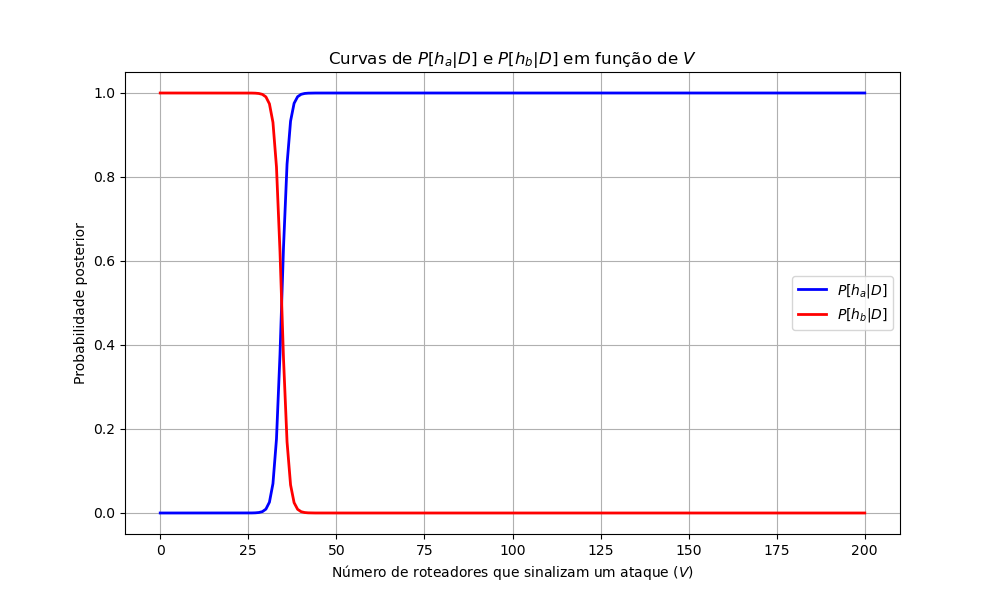
\includegraphics[width=\textwidth]{fig/item_7.png}
    \caption{Probabilidades \( P[h_a|D] \) e \( P[h_b|D] \) em função de \( V \) para \( P[h_a] = 0.1 \).}
    \label{fig:probabilidades}
\end{figure}

    \item Caso $P[h_a] = 0.1$, trace a curva $\log(P[h_a|D]/P[h_b|D])$ em função de $V$.
    
    \begin{tcolorbox}[colback=white, colframe=black, title=Resposta:]

    A curva \( \log(P[h_a|D]/P[h_b|D]) \) representa a relação logarítmica entre a probabilidade de um ataque estar ocorrendo em relação à probabilidade de não haver ataque, para diferentes valores de \( V \).
    
    Com \( P[h_a] = 0.1 \), a equação que devemos traçar é:
    $$
    \log\left( \frac{P[h_a|D]}{P[h_b|D]} \right) = \log\left( \frac{P[D|h_a] \cdot 0.1}{P[D|h_b] \cdot 0.9} \right) = \log\left( \frac{(0.24)^V (0.76)^{200 - V} \cdot 0.1}{(0.1)^V (0.9)^{200 - V} \cdot 0.9} \right)
    $$
    
    Podemos então traçar a curva dessa razão logarítmica, como visto na figura \ref{fig:log_probabilidades}. Conforme \( V \) aumenta, a razão \( P[h_a|D]/P[h_b|D] \) também aumenta, indicando uma maior confiança de que um ataque está ocorrendo.
    
\end{tcolorbox}

\begin{figure}[H]
    \centering
    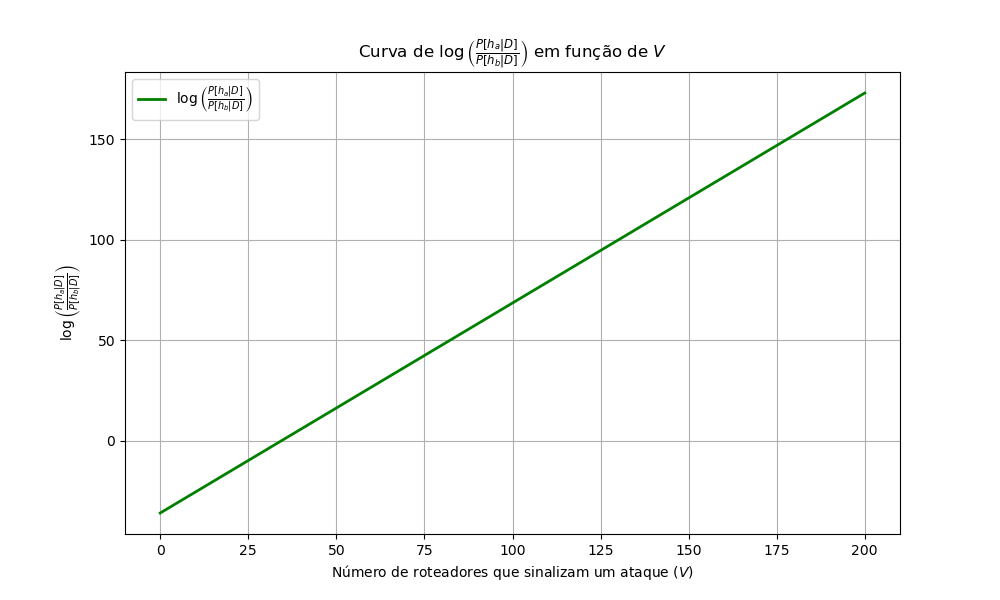
\includegraphics[width=\textwidth]{fig/item_8.png}
    \caption{Razão logarítmica entre \( P[h_a|D] \) e \( P[h_b|D] \) em função de \( V \) para \( P[h_a] = 0.1 \).}
    \label{fig:log_probabilidades}
\end{figure}

    \item Para $TPR = 0.9$ e $FPR = 0.1$, plote, em um mesmo gráfico, a função de probabilidade de massa:
    \begin{enumerate}
        \item do número de roteadores que alarmam quando há um ataque;
        \item do número de roteadores que alarmam quando não há um ataque.
    \end{enumerate}
    Na implementação do classificador central (aquele que recebe os sinais dos roteadores domésticos, e que são os “sensores” em cada residência), você deve decidir a partir de quantos roteadores residenciais alarmando o classificador central deverá detectar que um ataque está ocorrendo.
    \begin{enumerate}
        \item Explique como avaliar o erro da sua decisão.
        \item Estime esse erro para o valor escolhido.
    \end{enumerate}


    \begin{tcolorbox}[colback=white, colframe=black, title=Resposta:]

        Para \( TPR = 0.9 \) e \( FPR = 0.1 \), queremos traçar a função de probabilidade de massa (PMF) para o número de roteadores que alarmam em dois cenários:
        
        \begin{enumerate}
            \item Quando há um ataque (hipótese \( h_a \)),
            
            A função de probabilidade segue a distribuição binomial:
            $$
            P(V | h_a) = \binom{M}{V} (TPR)^V (1 - TPR)^{M - V}
            $$
            onde:
            \begin{itemize}
                \item \( M = 200 \) é o número total de roteadores,
                \item \( V \) é o número de roteadores que alarmam,
                \item \( TPR = 0.9 \) é a taxa de verdadeiros positivos, ou seja, a probabilidade de um roteador alarmar corretamente quando há um ataque.
            \end{itemize}
            
            Como \( TPR = 0.9 \), a maior parte dos roteadores deverá alarmar quando um ataque está ocorrendo, portanto a função de probabilidade de massa será concentrada em valores altos de \( V \), próximos a \( M \).

            \item Quando não há um ataque (hipótese \( h_b \)),
            
            Aqui, a distribuição binomial também é utilizada, mas com \( FPR = 0.1 \) (taxa de falsos positivos):
           $$
           P(V | h_b) = \binom{M}{V} (FPR)^V (1 - FPR)^{M - V}
           $$
           onde:
            \begin{itemize}
                \item \( M = 200 \) é o número total de roteadores,
                \item \( V \) é o número de roteadores que alarmam,
                \item \( FPR = 0.1 \) é a probabilidade de um roteador alarmar erroneamente quando não há ataque.
            \end{itemize}
           Como \( FPR = 0.1 \), esperamos que poucos roteadores alarmem no cenário sem ataque. Portanto, a função de probabilidade de massa será concentrada em valores baixos de \( V \), próximos de zero.
        \end{enumerate}
        
        \end{tcolorbox}

        \begin{tcolorbox}[colback=white, colframe=black, title=Resposta (continuação):]
        
        \textbf{Explicação do Gráfico:}
        
        O gráfico resultante (figura \ref{fig:pmf}) tem duas curvas:
        \begin{enumerate}
            \item A primeira curva, \( P(V | h_a) \), mostra a probabilidade de \( V \) roteadores alarmarem quando há um ataque. Como \( TPR = 0.9 \), a probabilidade será maior para valores altos de \( V \), indicando que muitos roteadores devem alarmar quando o ataque ocorre.
            \item A segunda curva, \( P(V | h_b) \), mostra a probabilidade de \( V \) roteadores alarmarem quando não há ataque. Como \( FPR = 0.1 \), a probabilidade será maior para valores baixos de \( V \), indicando que poucos roteadores alarmam quando não há ataque.
        \end{enumerate}

    \end{tcolorbox}

    \begin{figure}[H]
        \centering
        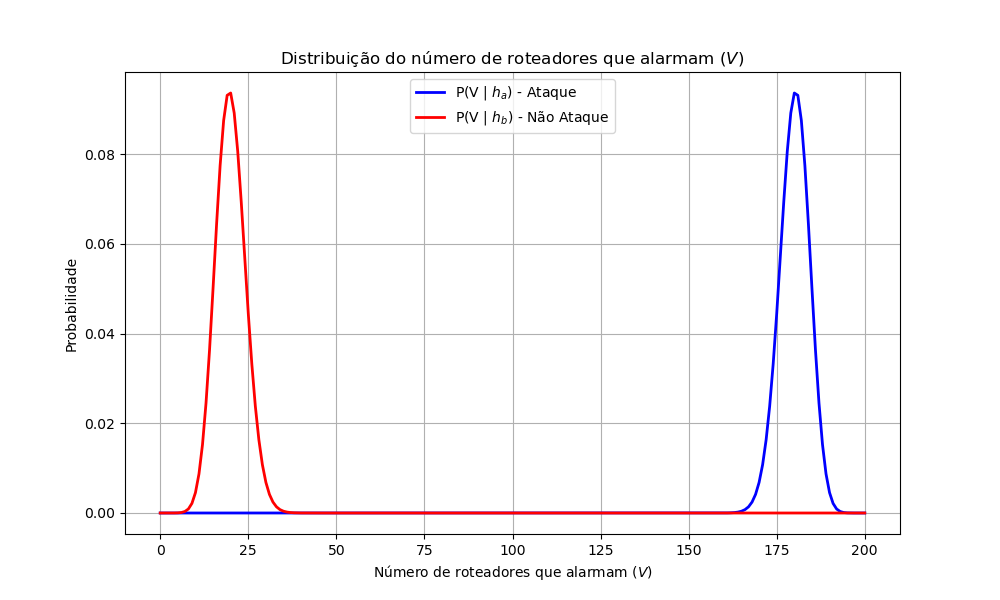
\includegraphics[width=\textwidth]{fig/item_9.png}
        \caption{Funções de probabilidade de massa (PMF) para o número de roteadores que alarmam.}
        \label{fig:pmf}
    \end{figure}

    \begin{tcolorbox}[colback=white, colframe=black, title=Resposta (continuação):]
        
        \textbf{Decisão do Limiar:}
        
        A partir do gráfico, podemos definir um limiar \( V_{\text{limiar}} \) que determina o número mínimo de roteadores alarmando necessário para que o classificador central conclua que um ataque está ocorrendo:
        \begin{itemize}
            \item Se \( V > V_{\text{limiar}} \), o classificador detecta um ataque.
            \item Se \( V \leq V_{\text{limiar}} \), o classificador conclui que não há ataque.
        \end{itemize}
        
        \textbf{Erro de Decisão:}
        
        O erro de decisão é composto por:
        \begin{itemize}
            \item Falsos positivos: ocorrem quando \( V > V_{\text{limiar}} \) no cenário sem ataque (\( h_b \)).
            \item Falsos negativos: ocorrem quando \( V \leq V_{\text{limiar}} \) no cenário com ataque (\( h_a \)).
        \end{itemize}
        
        A escolha do limiar \( V_{\text{limiar}} \) afeta diretamente a taxa de erro:

        \begin{itemize}
            \item Um limiar baixo aumenta os falsos positivos, pois mais alarmes serão registrados mesmo sem ataque.
            \item Um limiar alto aumenta os falsos negativos, pois pode haver um ataque, mas o número de alarmes não é suficiente para detectá-lo.
        \end{itemize}
        
        O ponto ideal de \( V_{\text{limiar}} \) deve ser escolhido de maneira a equilibrar os erros de decisão, minimizando falsos positivos e falsos negativos.
        
        \textbf{Estimativa do Erro:}
        
        Para um valor específico de \( V_{\text{limiar}} \), você pode estimar o erro somando:
        \begin{itemize}
            \item A probabilidade de falsos positivos \( P(V > V_{\text{limiar}} | h_b) \),
            \item A probabilidade de falsos negativos \( P(V \leq V_{\text{limiar}} | h_a) \).
        \end{itemize}

        Essas probabilidades são obtidas a partir das funções de probabilidade de massa traçadas anteriormente.
        
    
    \end{tcolorbox}


\end{enumerate}


%     \item O classificador central comete erros, evidentemente.
%     \begin{enumerate}
%         \item Calcule o $TPR_c$ e o $FPR_c$ do classificador central.
%         \item Plote a ROC curve do classificador central.
%         \item Compare o classificador central com o classificador residencial.
%     \end{enumerate}



% \begin{tcolorbox}[colback=white, colframe=black, title=Resposta:]

% (a) O \( TPR_c \) (taxa de verdadeiros positivos do classificador central) e o \( FPR_c \) (taxa de falsos positivos) podem ser calculados usando os limiares que escolhemos para detectar ataques. Se o classificador central detecta um ataque quando \( V \) roteadores alarmam, então:
% $$
% TPR_c = P(V \geq \text{limiar} | h_a)
% $$
% e
% $$
% FPR_c = P(V \geq \text{limiar} | h_b)
% $$

% (b) A ROC curve (Receiver Operating Characteristic) é traçada plotando \( TPR_c \) contra \( FPR_c \) para diferentes limiares. Quanto maior o \( TPR_c \) para um dado \( FPR_c \), melhor é o desempenho do classificador central.

% (c) O classificador central tende a ser mais confiável que os classificadores residenciais individuais, pois agrega as decisões de múltiplos roteadores. Isso reduz o impacto de falsos positivos e falsos negativos individuais, melhorando a detecção geral do sistema.




\end{document}